\documentclass[11pt,a4paper]{article}
\usepackage{fontspec}
\setmainfont{TeX Gyre Pagella}
\newfontfamily\headfont{Inter}[UprightFont=*-ExtraBold,BoldFont=*-ExtraBold,Extension=.otf,Path=/usr/share/fonts/opentype/inter/]
\usepackage[a4paper,margin=2.3cm]{geometry}
\usepackage{graphicx,booktabs,float,caption,array,xcolor,longtable}
\usepackage{xurl}
\usepackage[hidelinks]{hyperref}
\usepackage{titlesec}
\usepackage[round]{natbib}
\usepackage{setspace}
\setstretch{1.05}
\renewcommand{\topfraction}{0.9}
\renewcommand{\bottomfraction}{0.8}
\renewcommand{\textfraction}{0.1}
\renewcommand{\floatpagefraction}{0.75}
\setlength{\parindent}{0pt}
\setlength{\emergencystretch}{2em}
\setlength{\parskip}{0.55em}
\titleformat{\section}{\headfont\Large}{\thesection}{0.8em}{}
\titleformat{\subsection}{\headfont\large}{\thesubsection}{0.8em}{}
\captionsetup{font=small,labelfont=bf}
\urlstyle{same}
\hypersetup{pdftitle={The World's Tallest Building},pdfauthor={Tristan Hotham}}

\begin{document}
\begin{center}
{\Large\bfseries The World's Tallest Building\par}
\vspace{0.4em}
{\large Who held the record, for how long, and where today's tall buildings are,\\from the Great Pyramid to Jeddah Tower\par}
\vspace{1.2em}
{\large Tristan Hotham\par}
\vspace{0.3em}
{\small Independent researcher\\
ORCID: 0000-0003-4931-9349\\
DOI: https://doi.org/10.5281/zenodo.23857608\par}
\vspace{0.8em}
2026
\end{center}

\begin{quote}
\small
\begin{center}\textbf{Abstract}\end{center}
The title of the world's tallest building is easy to name today and surprisingly slippery in the past, because it depends on what counts as a building and how height is measured. Using the record-holder tables of English Wikipedia's history of the world's tallest buildings, its list of the 98 buildings of 350 m or more, and a cleaned extract of Wikidata, I trace the record from the Great Pyramid of Giza to the Burj Khalifa and map today's tall buildings. Treating churches as buildings, as the source does, the record has been held in 15 cities since the 13th century. Lincoln Cathedral held it longest, 238 years from 1311 to 1549, and churches held it for 583 of the 715 years since 1311 (82\%). New York held it for 65 years and the United States for 104, until the Petronas Towers took it to Kuala Lumpur in 1998; it has stayed in Asia since. The Great Pyramid, a structure rather than a building, was the tallest structure for about 3,870 years. Of the 98 buildings of 350 m or more, 81 (83\%) are in Asia and 82 were finished since 2010. Among 464 buildings of 200 m or more in Wikidata that survive unit checks, Asia's share of completions rose from 27\% in the 1980s to 75\% in the 2010s. Wikipedia lists Jeddah Tower as under construction at a planned 1,008 m, with completion planned for 2028. I set out the definitions each source uses and the unit errors in Wikidata's heights, which make naive counts of tall buildings unreliable.

\textbf{Keywords:} tallest buildings; skyscrapers; history of architecture; cathedrals; CTBUH; Wikidata; Wikipedia; data quality; maps
\end{quote}

\section{Introduction}
Few records are as public as the world's tallest building. It has been claimed by cathedral chapters, insurance companies, banks, oil states and developers, argued over in newspapers and settled, since the late 20th century, by the Council on Tall Buildings and Urban Habitat (CTBUH) and its measurement rules \citep{ctbuh}. English Wikipedia keeps a history of the record, with tables of the holders and their heights, and a list of the tallest buildings standing now \citep{wphist,wplist}. Wikidata, the structured sister project, records heights, coordinates and dates for thousands of buildings \citep{wikidata}.

This paper puts those sources together to answer three descriptive questions. Which buildings and cities held the record, and for how long? How did the building of very tall towers spread across the world, and when did Asia overtake North America? And where are today's tall buildings? An interactive version, with a slider that follows the record through time over a map of today's buildings, is at \url{https://maps.tristanhotham.com/tallest-buildings/}.

\section{Definitions}
The answer depends on the definition, and the sources use three.

\textbf{Buildings in the history of the record.} Wikipedia's history page defines a building as something regularly inhabited or occupied, cites the CTBUH's definition of a building as a structure ``designed for residential, business or manufacturing purposes'' that ``has floors'', and says that it ``treats churches and cathedrals as buildings'', although much of their height is in towers and spires that are not occupied \citep{wphist}. Heights follow the CTBUH default, the architectural top, including spires but not antennas, masts or flagpoles. The page notes that the CTBUH adopted three criteria in 1996, when the Petronas Towers and the Sears Tower disputed the title; by the highest tip, the Sears Tower kept the record until 2010.

\textbf{Today's tallest buildings.} The list page counts ``enclosed structures with continuously occupiable floors'' of at least 350 m to the highest architectural feature, completed or architecturally topped out, and excludes non-building structures such as radio towers \citep{wplist}. In the revision used it has 98 entries.

\textbf{Structures.} The Great Pyramid of Giza, the Washington Monument (169 m, 1884), the Eiffel Tower (300 m, 1889) and from 1954 a succession of radio and television masts held the record for the tallest structure of any kind without being buildings. According to the history page, since 1884 the tallest structure has also been the tallest building only from 1930 to 1954 and since 2010.

I keep two tracks throughout: the tallest building, which follows the history page's tables, and the tallest structure, which follows its text.

\section{Data}
\textbf{Record-holders.} The history page \citep{wphist} has a table of 10 rows for churches and cathedrals (13th century to 1894) and one of 12 rows for skyscrapers (1894 to the present), with years held, city, height and, for skyscrapers, status. Together they name 21 buildings, as St Mary's Church in Stralsund held the title twice. The structures track uses the page's prose for the Great Pyramid (146.5 m, ``the tallest structure in the world for over 3,800 years, until the construction of Lincoln Cathedral in 1311''), the Washington Monument, the Eiffel Tower, the Chrysler and Empire State Buildings, the masts from 1954 and the Burj Khalifa from 2010. The page gives no date for the Great Pyramid; I use Wikidata's inception, 2560 BC, which is consistent with the page's ``over 3,800 years''.

\textbf{Today's tallest.} The list page \citep{wplist} gives name, height, floors, city, country and year for the 98 buildings of 350 m or more, 46 buildings of 350 m or more under construction, and the tallest building on each continent.

\textbf{Wikidata.} An extract of 4,669 Wikidata items that are architectural structures with a height of 100 or more (7,395 rows, one per class), with coordinates, official opening, inception, city, country and class \citep{wikidata}. Heights were extracted without their units.

\textbf{Checks and geography.} For buildings in the United States I compared heights with the CORGIS skyscrapers dataset, a teaching dataset of about 2,400 United States buildings derived from the CTBUH Skyscraper Center to 2016 \citep{corgis}. It is used only to check units and is not redistributed. Countries, regions and city names come from Natural Earth \citep{naturalearth}.

\begin{table}[tbp]\centering\small\caption{Sources, what was used and licences.}\label{tab:sources}\begin{tabular}{>{\raggedright\arraybackslash}p{3.6cm}>{\raggedright\arraybackslash}p{7.2cm}>{\raggedright\arraybackslash}p{2.6cm}}\toprule Source & Used for & Licence\\\midrule
Wikipedia, History of the world's tallest buildings & 22 record-holder rows; definitions; structures in the text & CC BY-SA 4.0\\
Wikipedia, List of tallest buildings & 98 buildings of 350 m or more; 46 under construction & CC BY-SA 4.0\\
Wikidata & 4,669 structures of height 100 or more; 1,343 buildings kept & CC0\\
CORGIS skyscrapers & Unit check for United States heights only & GPL-3.0 (not redistributed)\\
Natural Earth & Countries, regions, city names & Public domain\\
\bottomrule\end{tabular}\end{table}

\section{Methods}
\textbf{Years held.} Each holder's reign runs from its first year to the next holder's, with 2026 as the end of the Burj Khalifa's reign so far. Old St Paul's Cathedral's reign has no start (``13th century''), so I leave London out of the totals. Years are summed by city and by present-day country.

\textbf{Cleaning Wikidata.} The steps, in order, are:
\begin{enumerate}
\item Keep items whose classes include a kind of occupied building (skyscraper, tower block, office, hotel, residential or apartment building, civic and commercial buildings, churches, mosques and temples) and drop those that are also towers, masts, transmitters, bridges, dams, monuments and similar unless they are also skyscrapers or offices (2,543 items dropped).
\item Drop items classed as under construction, unfinished or destroyed (29) and heights over 830 m, taller than the Burj Khalifa and so certainly in the wrong unit (11).
\item Where an item has two heights about 3.28 apart, keep the smaller (metres).
\item Buildings of 350 m or more must match the list page, by name, alias or height and city; matched items take the list's height, year and city (83 matched), and Wikidata items of 350 m or more not on it are dropped (99). The 13 list buildings missing from the extract are added at their city centre.
\item Drop items with no opening or inception year, or one after 2026 (319).
\item United States: keep a height under 350 m only if a CORGIS building of the same name within 30 km has a height within 8\%. 156 agreed, 14 disagreed (4 of them by the ratio of feet to metres) and 242 could not be checked; only the 156 are counted.
\item Elsewhere, keep heights as given, except 4 found on reading the list of buildings of 200 m or more to be plainly feet (a cathedral founded in 1075 at 277 m, for example).
\item Leave the 82 churches, mosques and temples out of the counts and the map, because Wikidata dates them by their founding rather than by when they reached their height.
\end{enumerate}
The result is 1,343 buildings of 100 m or more, 464 of them 200 m or more. The year is the official opening where Wikidata has one (426 buildings), otherwise the inception (819), and the list's year for list buildings (98).

\textbf{Regions and cities.} Points are placed in Natural Earth countries and grouped into nine regions from Natural Earth subregions (Hong Kong, Macau and Taiwan with East Asia; Western Asia, including Turkey, as the Middle East; Central Asia with South Asia). ``Asia'' means East, Southeast and South Asia and the Middle East. A building's city is the largest Natural Earth populated place of 400,000 or more within 40 km, unless a place of 150,000 or more is less than a third as far away, otherwise the nearest place within 30 km. Static maps use the Equal Earth projection \citep{equalearth}.

\section{Results}
\subsection{The record-holders}
Figure~\ref{fig:skyline} draws every holder to scale and Table~\ref{tab:records} lists them. The first building in the history page's table is Old St Paul's Cathedral in London (149 m). Lincoln Cathedral took the title in 1311 with a spire of 159.7 m and held it until the spire collapsed in 1549. Collapse and fire then passed it between St Mary's in Stralsund, Beauvais Cathedral and Strasbourg Cathedral, which held it from 1647 to 1874 at 142 m, the lowest of any holder. Hamburg, Rouen, Cologne and Ulm followed between 1874 and 1890; Ulm Minster (161.5 m) was the last church to hold the record. Philadelphia City Hall (167 m) took it in 1894, and from 1908 to 1973 it stayed in New York: the Singer Building, the Metropolitan Life Tower, the Woolworth Building, 40 Wall Street and the Chrysler Building (both 1930), the Empire State Building (381 m, 39 years) and the World Trade Center (417 m). The Sears Tower in Chicago (442 m) held it from 1973 to 1998, the Petronas Towers (452 m) to 2004, Taipei 101 (510 m) to 2010, and the Burj Khalifa (828 m) since. The Burj Khalifa's margin over Taipei 101, 318 m or 62\%, is the largest increase in the record's history.

\begin{figure}[tbp]\centering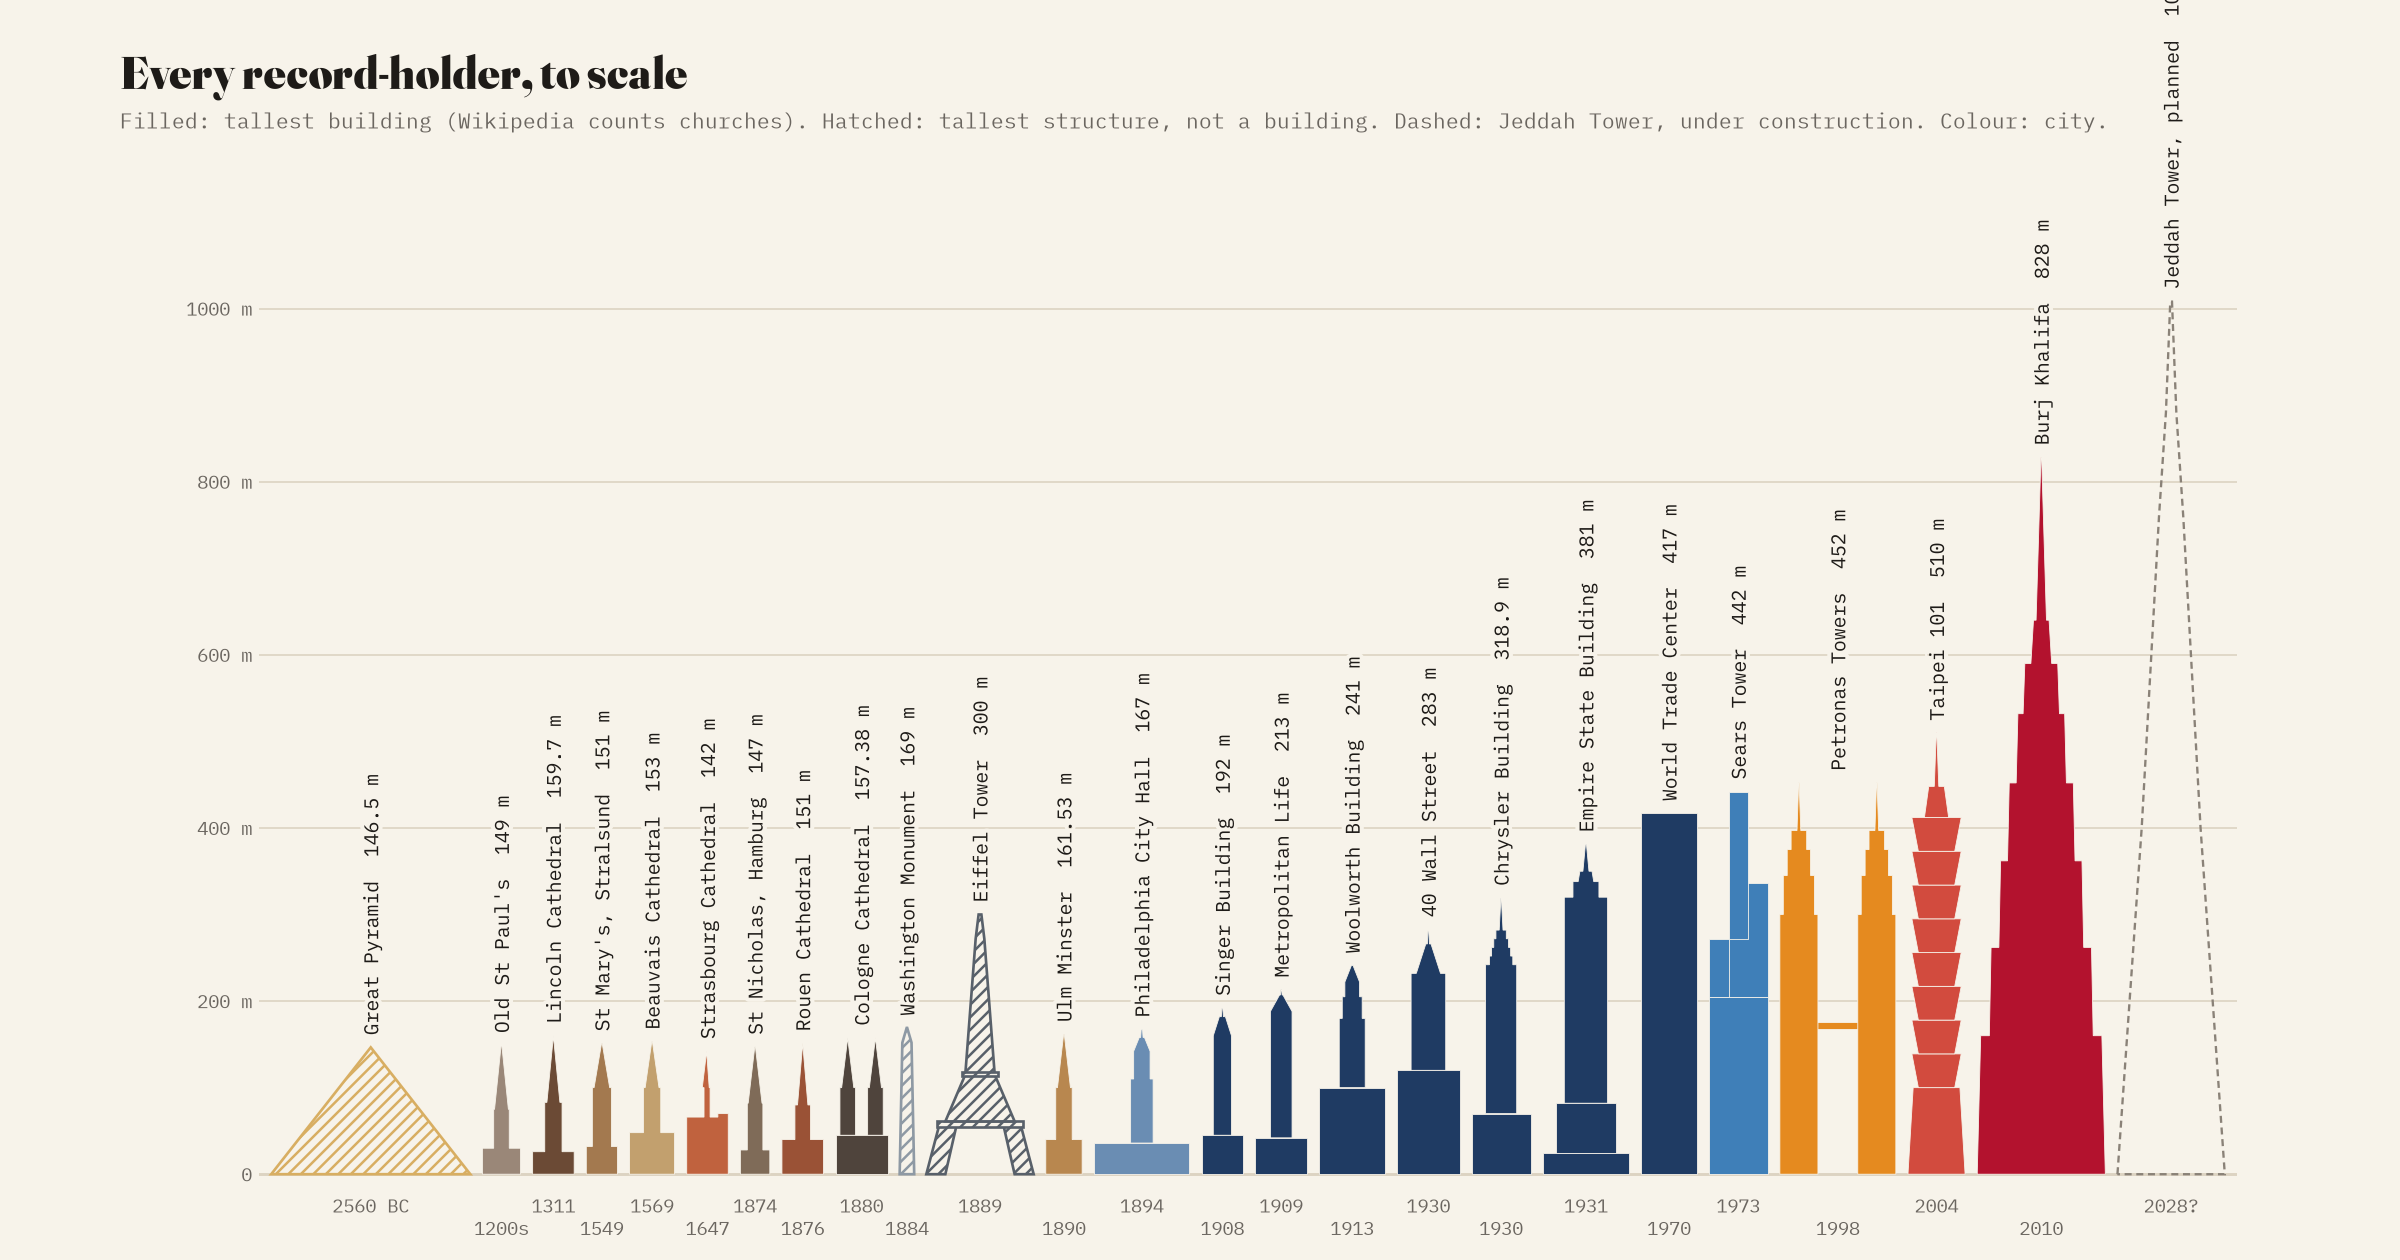
\includegraphics[width=\textwidth]{f_skyline.png}
\caption{Every holder of the record, to scale and in order. Filled: tallest building (churches count, as in the source); hatched: tallest structure that was not a building; dashed: Jeddah Tower, under construction. Heights from the Wikipedia tables; outlines are simplified sketches.}\label{fig:skyline}\end{figure}

\begin{table}[tbp]\centering\small\caption{Holders of the title of world's tallest building (Wikipedia's tables; churches count as buildings). Years to 2026 for the Burj Khalifa.}\label{tab:records}\setlength{\tabcolsep}{4pt}\begin{tabular}{l>{\raggedright\arraybackslash}p{5.2cm}>{\raggedright\arraybackslash}p{2.6cm}rr}\toprule Years & Building & City & Height (m) & Years held\\\midrule
13th century to 1311 & Old St Paul's Cathedral & London & 149 & \\
1311 to 1549 & Lincoln Cathedral & Lincoln & 159.7 & 238\\
1549 to 1569 & St. Mary's Church & Stralsund & 151 & 20\\
1569 to 1573 & St. Pierre's Cathedral & Beauvais & 153 & 4\\
1573 to 1647 & St. Mary's Church & Stralsund & 151 & 74\\
1647 to 1874 & Cathedral of Our Lady of Strasbourg & Strasbourg & 142 & 227\\
1874 to 1876 & Church of St. Nicholas & Hamburg & 147 & 2\\
1876 to 1880 & Rouen Cathedral & Rouen & 151 & 4\\
1880 to 1890 & Cologne Cathedral & Cologne & 157.38 & 10\\
1890 to 1894 & Ulm Minster & Ulm & 161.53 & 4\\
1894 to 1908 & Philadelphia City Hall & Philadelphia & 167 & 14\\
1908 to 1909 & Singer Building & New York City & 192 & 1\\
1909 to 1913 & Metropolitan Life Tower & New York City & 213 & 4\\
1913 to 1930 & Woolworth Building & New York City & 241 & 17\\
1930 to 1930 & 40 Wall Street & New York City & 283 & 0\\
1930 to 1931 & Chrysler Building & New York City & 318.9 & 1\\
1931 to 1970 & Empire State Building & New York City & 381 & 39\\
1970 to 1973 & 1 World Trade Center & New York City & 417 & 3\\
1973 to 1998 & Sears Tower & Chicago & 442 & 25\\
1998 to 2004 & Petronas Towers & Kuala Lumpur & 452 & 6\\
2004 to 2010 & Taipei 101 & Taipei & 510 & 6\\
2010 to present & Burj Khalifa & Dubai & 828 & 16\\
\bottomrule\end{tabular}\end{table}

\subsection{How long each city held it}
Figure~\ref{fig:tenure} and Table~\ref{tab:cities} show the years held. Lincoln (238 years) and Strasbourg (227) dominate, then Stralsund (94), New York (65), Chicago (25), Dubai (16 so far) and Philadelphia (14). By present-day country the United Kingdom leads with 238 years, France 235, Germany 110 and the United States 104. Churches held the title for 583 of the 715 years since 1311 (82\%). The history page's introduction says New York held the record for 86 years and Chicago for 30; its own table gives 65 and 25, which I use. The list page also says Strasbourg Cathedral was the tallest building from 1439 to 1874, while the history table gives 1647 to 1874.

\begin{figure}[tbp]\centering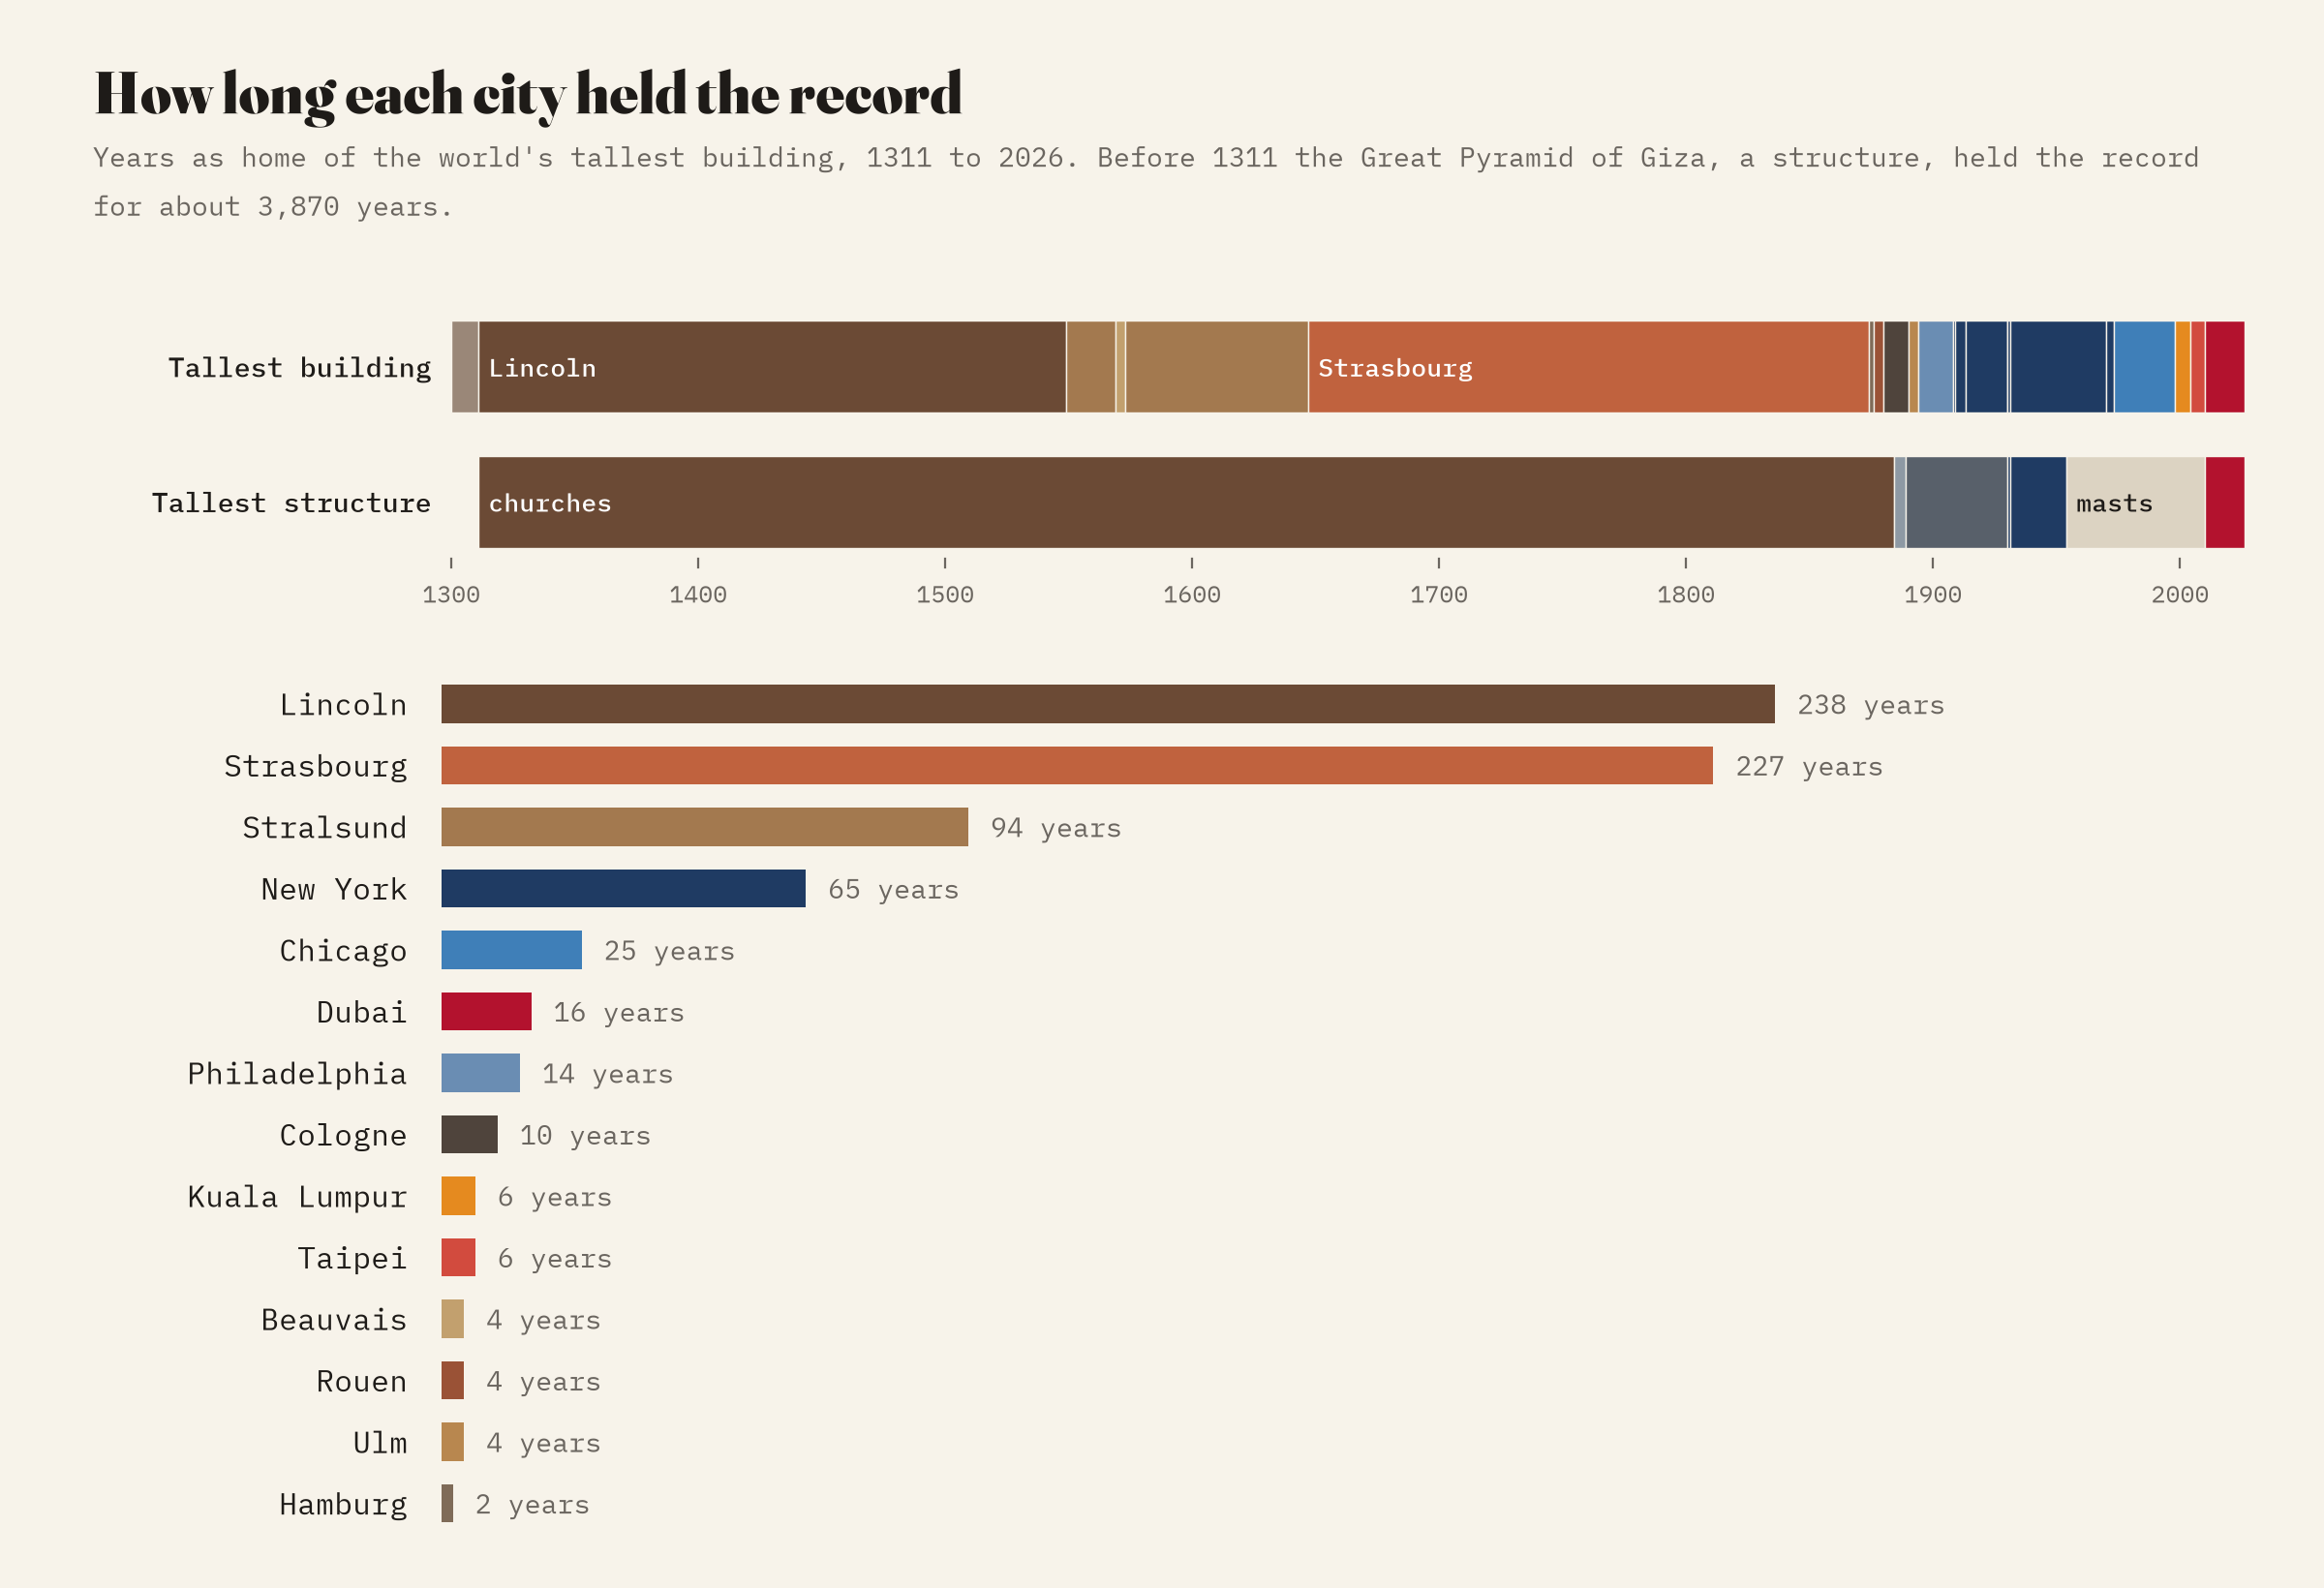
\includegraphics[width=\textwidth]{f_tenure.png}
\caption{Top: the tallest building and the tallest structure, 1300 to 2026, coloured by city. Bottom: years as home of the tallest building, by city.}\label{fig:tenure}\end{figure}
\begin{figure}[tbp]\centering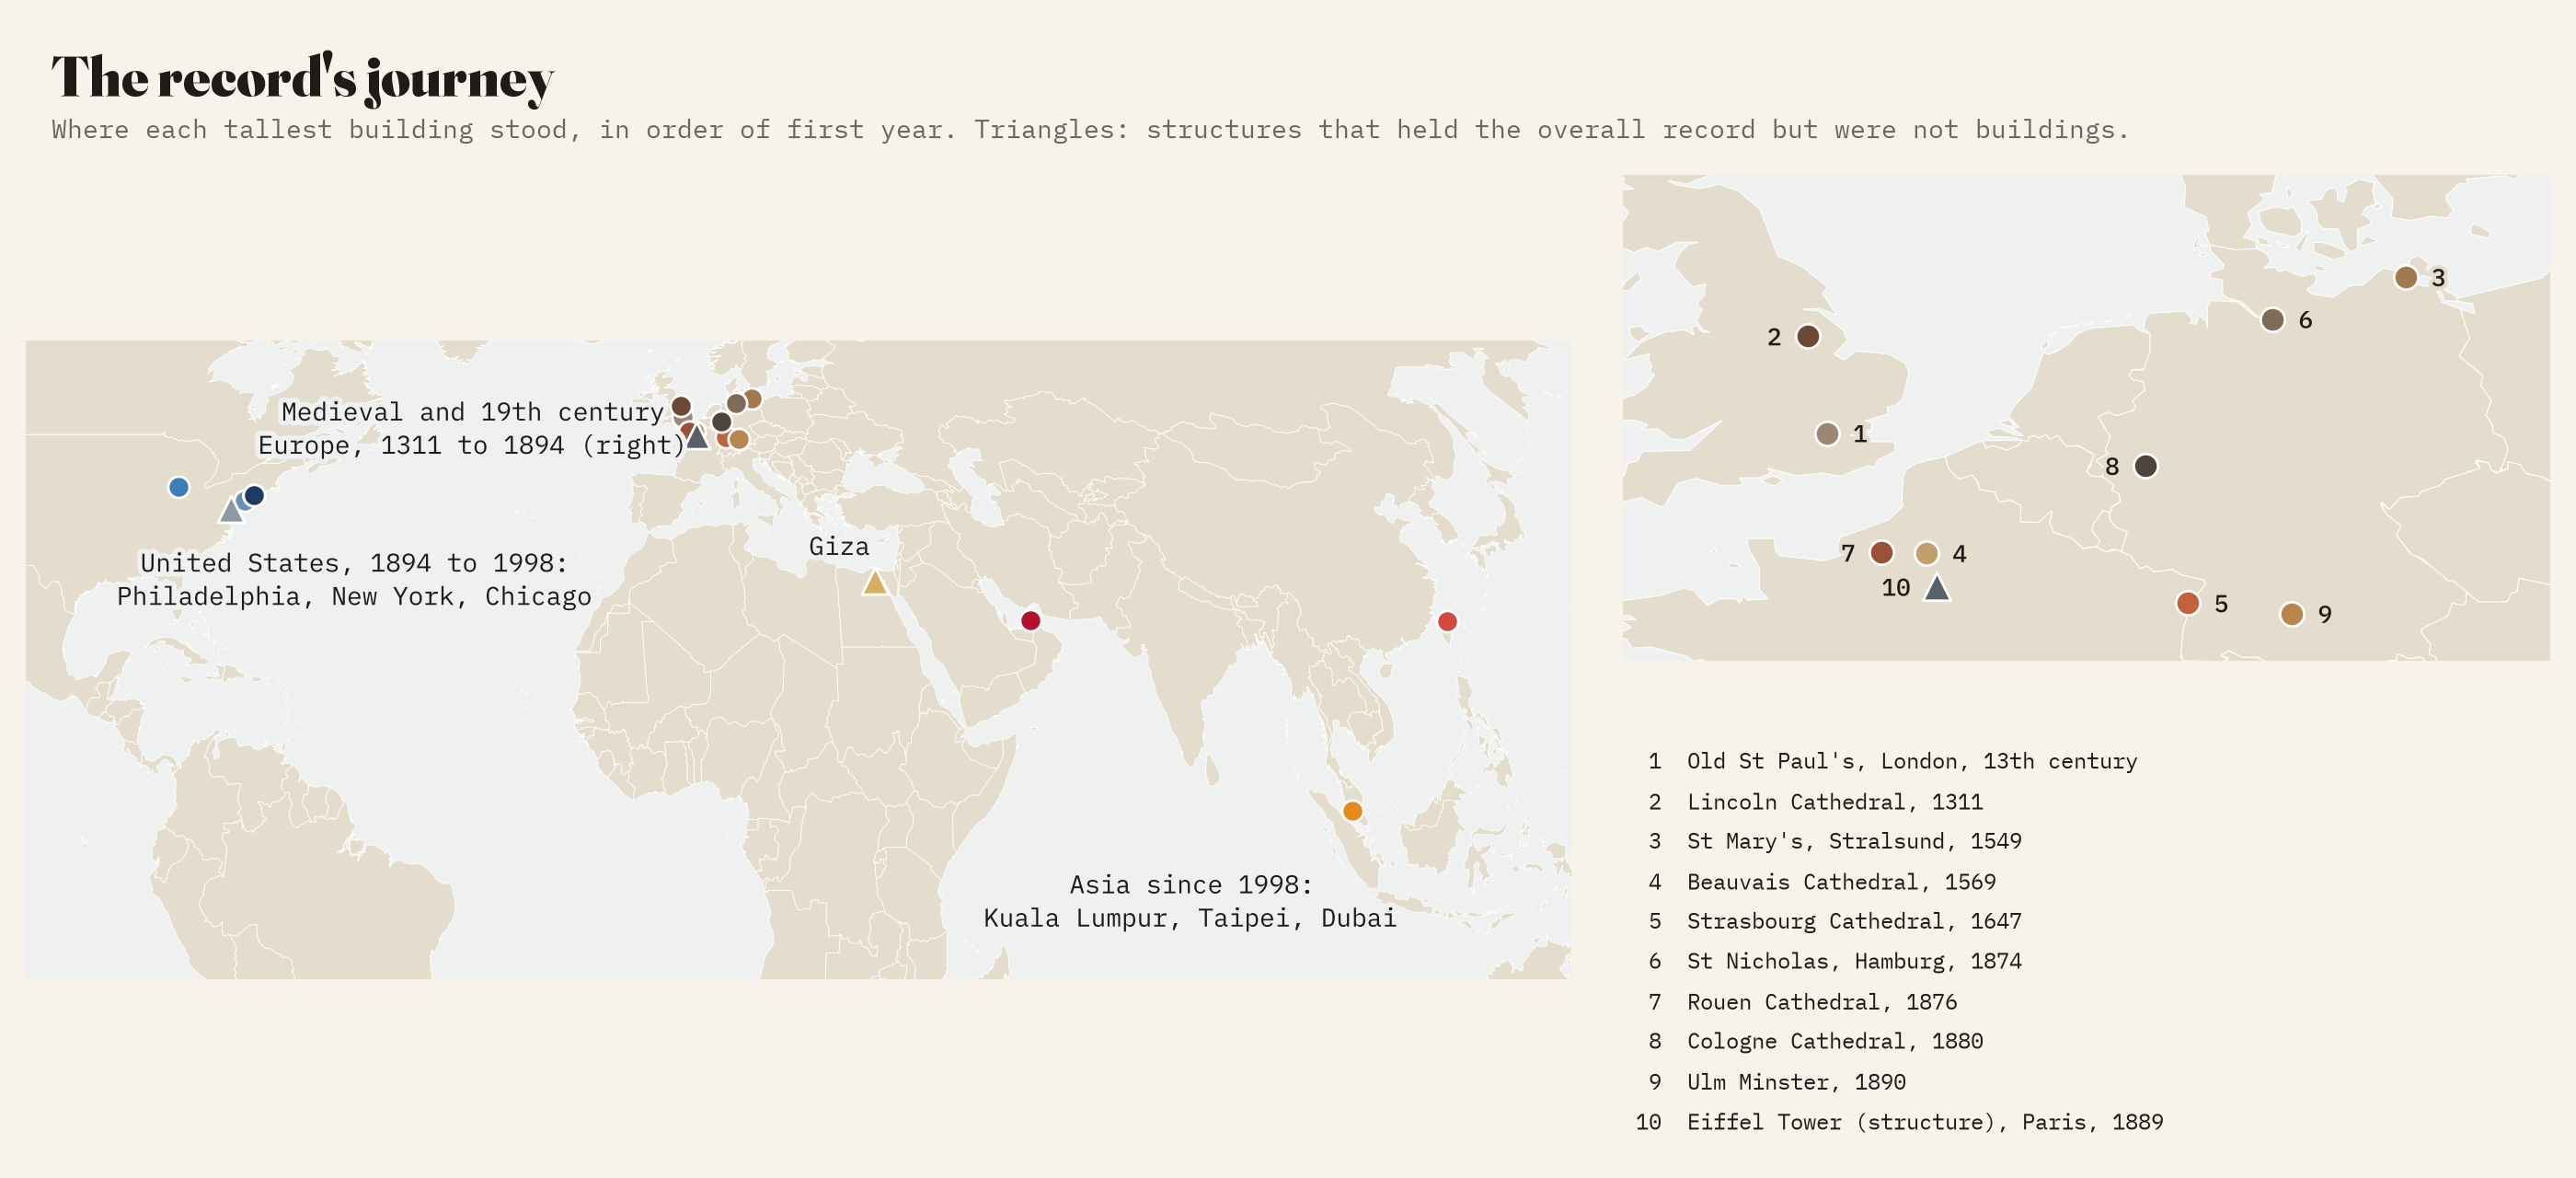
\includegraphics[width=\textwidth]{f_route.png}
\caption{Where the record-holders stood. Triangles: the Great Pyramid, the Washington Monument and the Eiffel Tower, which held the record for structures but were not buildings.}\label{fig:route}\end{figure}

\begin{table}[tbp]\centering\small\caption{Years as home of the world's tallest building, 1311 to 2026, by city.}\label{tab:cities}\begin{tabular}{llr>{\raggedright\arraybackslash}p{6.4cm}}\toprule City & Country & Years & Buildings\\\midrule
Lincoln & United Kingdom & 238 & Lincoln Cathedral\\
Strasbourg & France & 227 & Cathedral of Our Lady of Strasbourg\\
Stralsund & Germany & 94 & St. Mary's Church\\
New York & United States & 65 & 1 World Trade Center; 40 Wall Street; Chrysler Building; Empire State Building; Metropolitan Life Tower; Singer Building; Woolworth Building\\
Chicago & United States & 25 & Sears Tower\\
Dubai & United Arab Emirates & 16 & Burj Khalifa\\
Philadelphia & United States & 14 & Philadelphia City Hall\\
Cologne & Germany & 10 & Cologne Cathedral\\
Kuala Lumpur & Malaysia & 6 & Petronas Towers\\
Taipei & Taiwan & 6 & Taipei 101\\
Beauvais & France & 4 & St. Pierre's Cathedral\\
Rouen & France & 4 & Rouen Cathedral\\
Ulm & Germany & 4 & Ulm Minster\\
Hamburg & Germany & 2 & Church of St. Nicholas\\
\bottomrule\end{tabular}\end{table}

\subsection{The boom and the move to Asia}
Of the 464 buildings of 200 m or more, 355 (77\%) were finished in 2000 or later and 212 in the 2010s alone (Figure~\ref{fig:boom}). Before 1990, 73\% were in North America and 13\% in Asia. Asia's share of completions rose from 27\% in the 1980s to 52\% in the 1990s, 63\% in the 2000s and 75\% in the 2010s; the 2020s so far stand at 75\%. Because unchecked United States records are left out, North America is undercounted. Counting all 95 unchecked United States records of 200 m or more, many of which are certainly feet, Asia's share in the 2010s would still be 65\%.

The complete list of buildings of 350 m or more shows the same shift more sharply. 81 of the 98 (83\%) are in Asia: 55 in East Asia, 20 in the Middle East and 6 in Southeast Asia, against 13 in North America, 3 in Europe and 1 in Africa. Only 9 were finished before 2000; 82 were finished in 2010 or later. The oldest is the Empire State Building of 1931.

\begin{figure}[tbp]\centering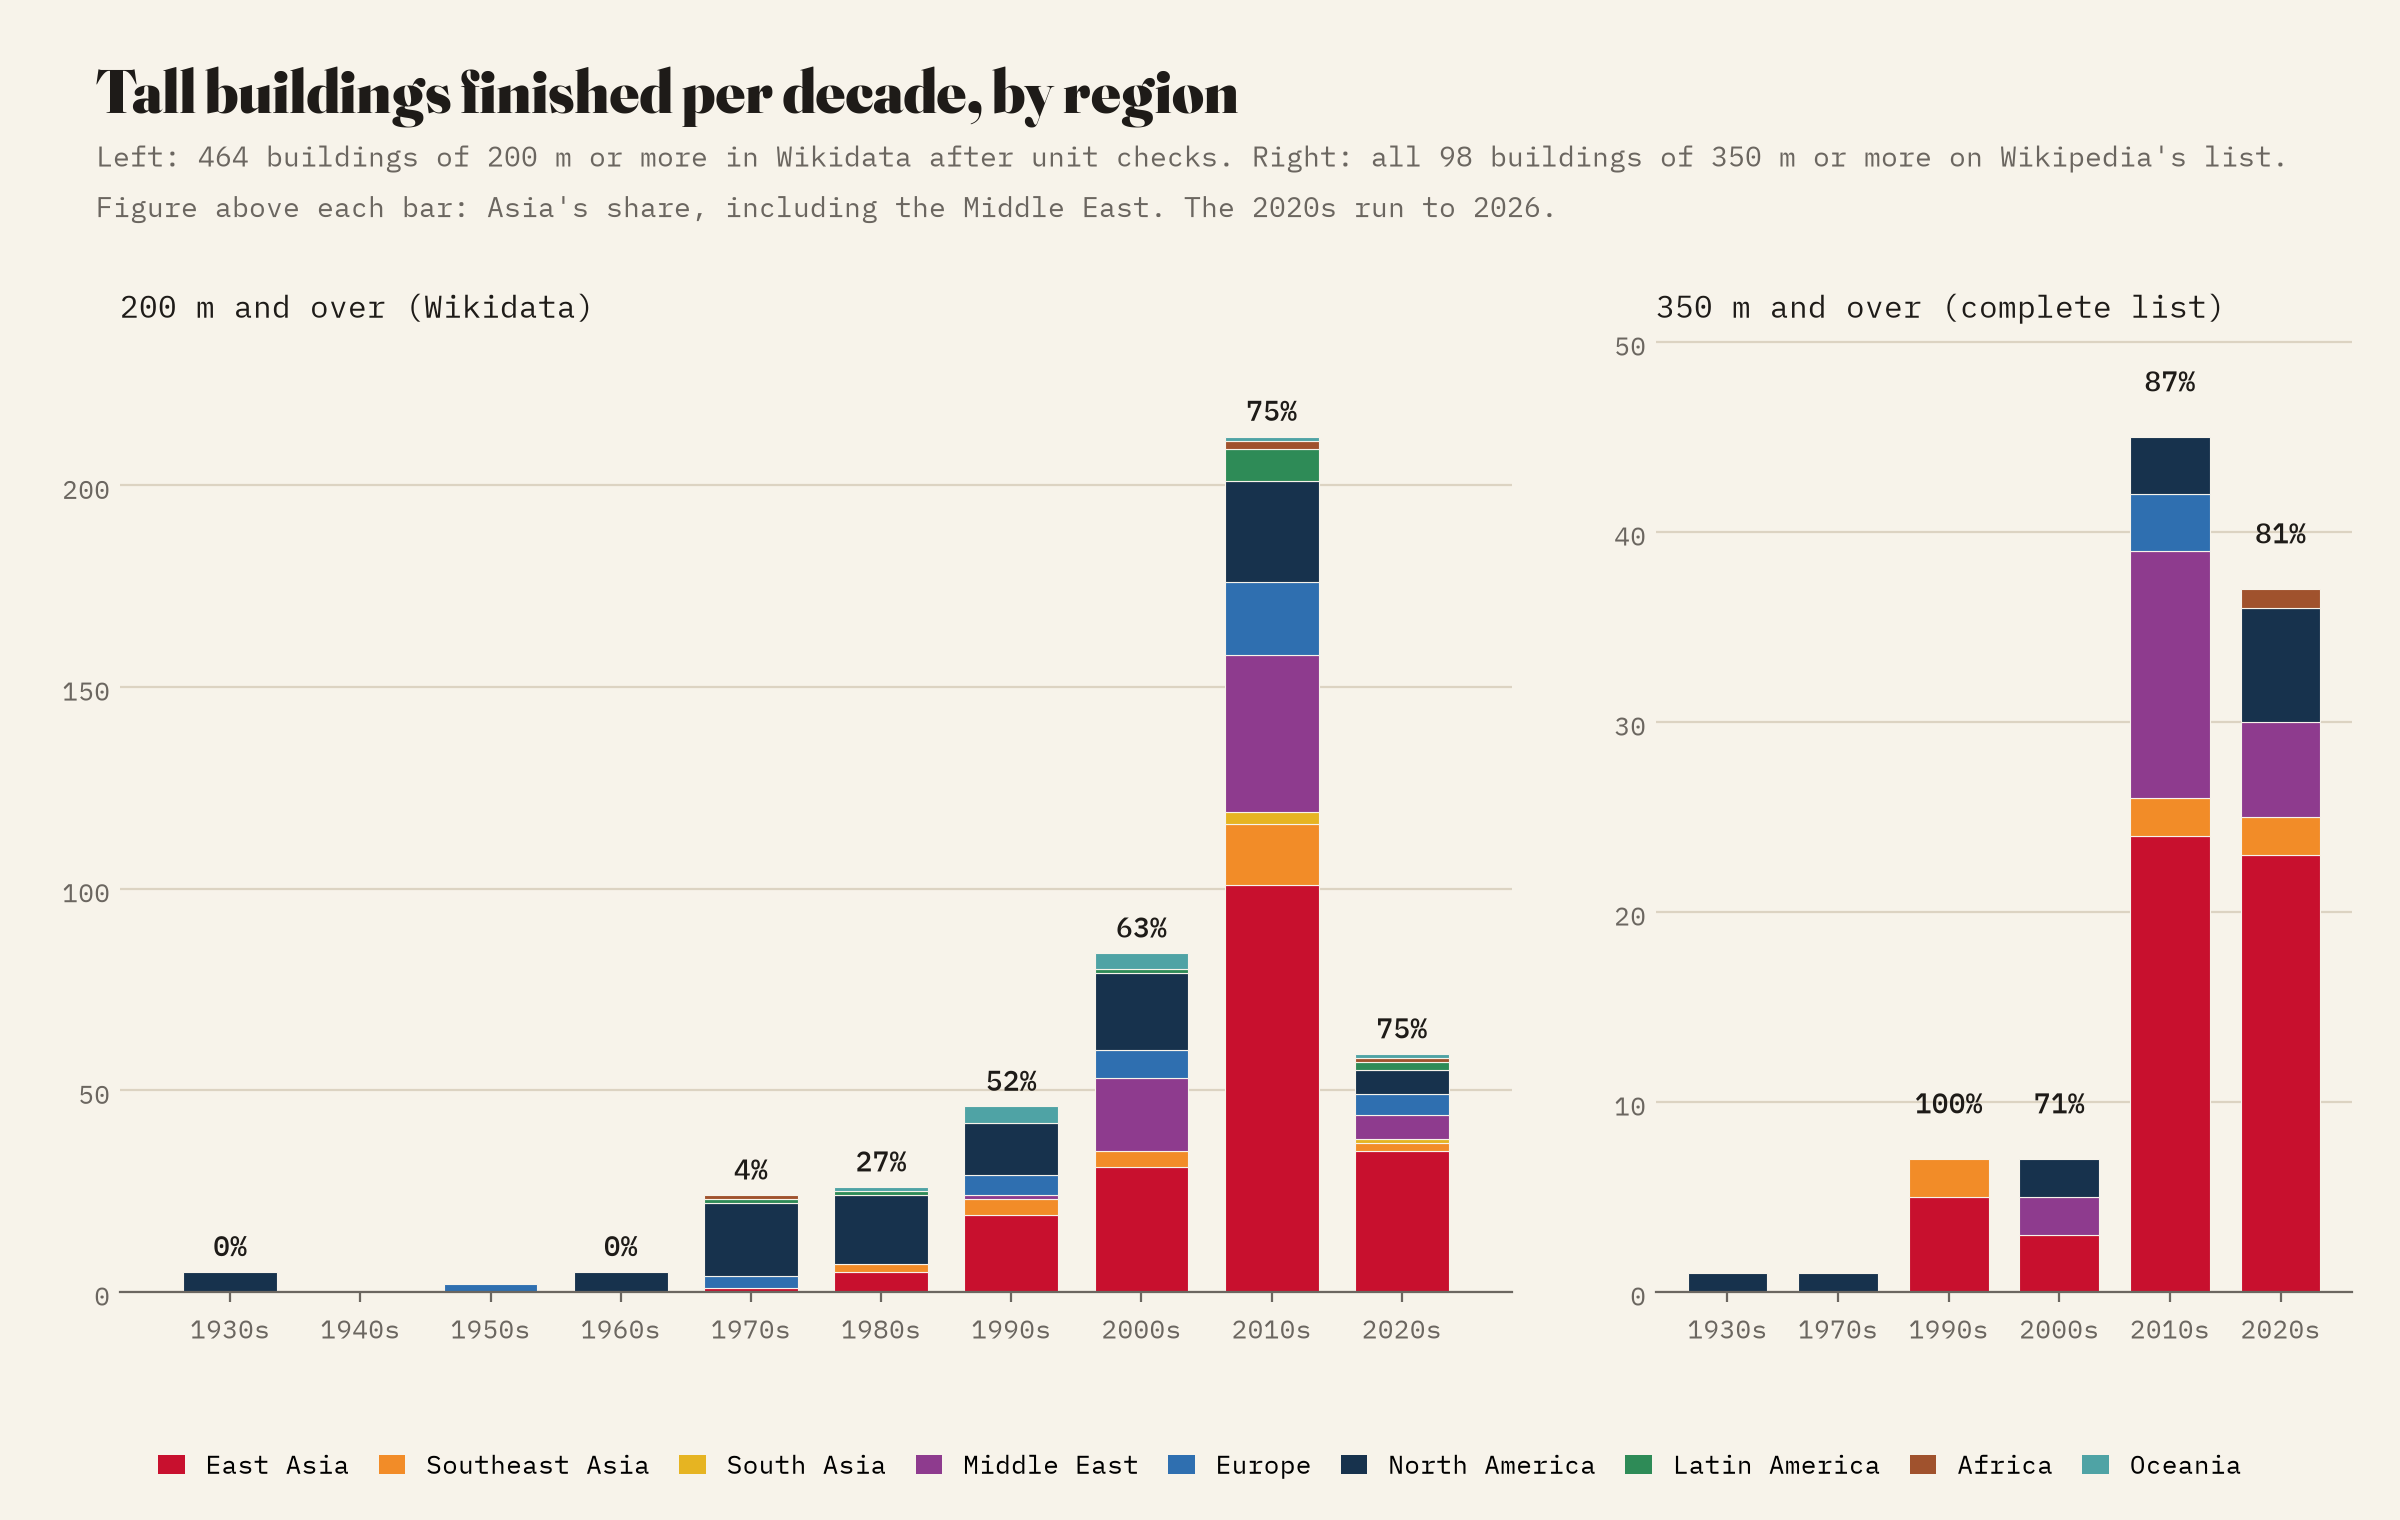
\includegraphics[width=\textwidth]{f_boom.png}
\caption{Buildings finished per decade by region: 200 m or more in Wikidata after unit checks (left) and all buildings of 350 m or more on Wikipedia's list (right). Figures above the bars: Asia's share, including the Middle East.}\label{fig:boom}\end{figure}

\subsection{Where they are now}
Wikidata, after the checks, has the most buildings of 200 m or more in New York (43), Dubai (37), Shenzhen (36), Chicago (18) and Tokyo (16) (Figures~\ref{fig:map} and \ref{fig:cities}, Table~\ref{tab:top}). These are counts of records. Wikidata is patchy for China: 10 of the list's 52 buildings of 350 m or more in China and Hong Kong (19\%) are missing from the extract, against 3 of the other 46 (7\%), and coverage of shorter buildings is likely to be worse. For the very tallest, the complete list is the better guide: it puts Dubai first with 15 buildings of 350 m or more, then Shenzhen (12) and New York (9). By country, the list has 48 buildings in mainland China, 16 in the United Arab Emirates and 12 in the United States.

\begin{figure}[tbp]\centering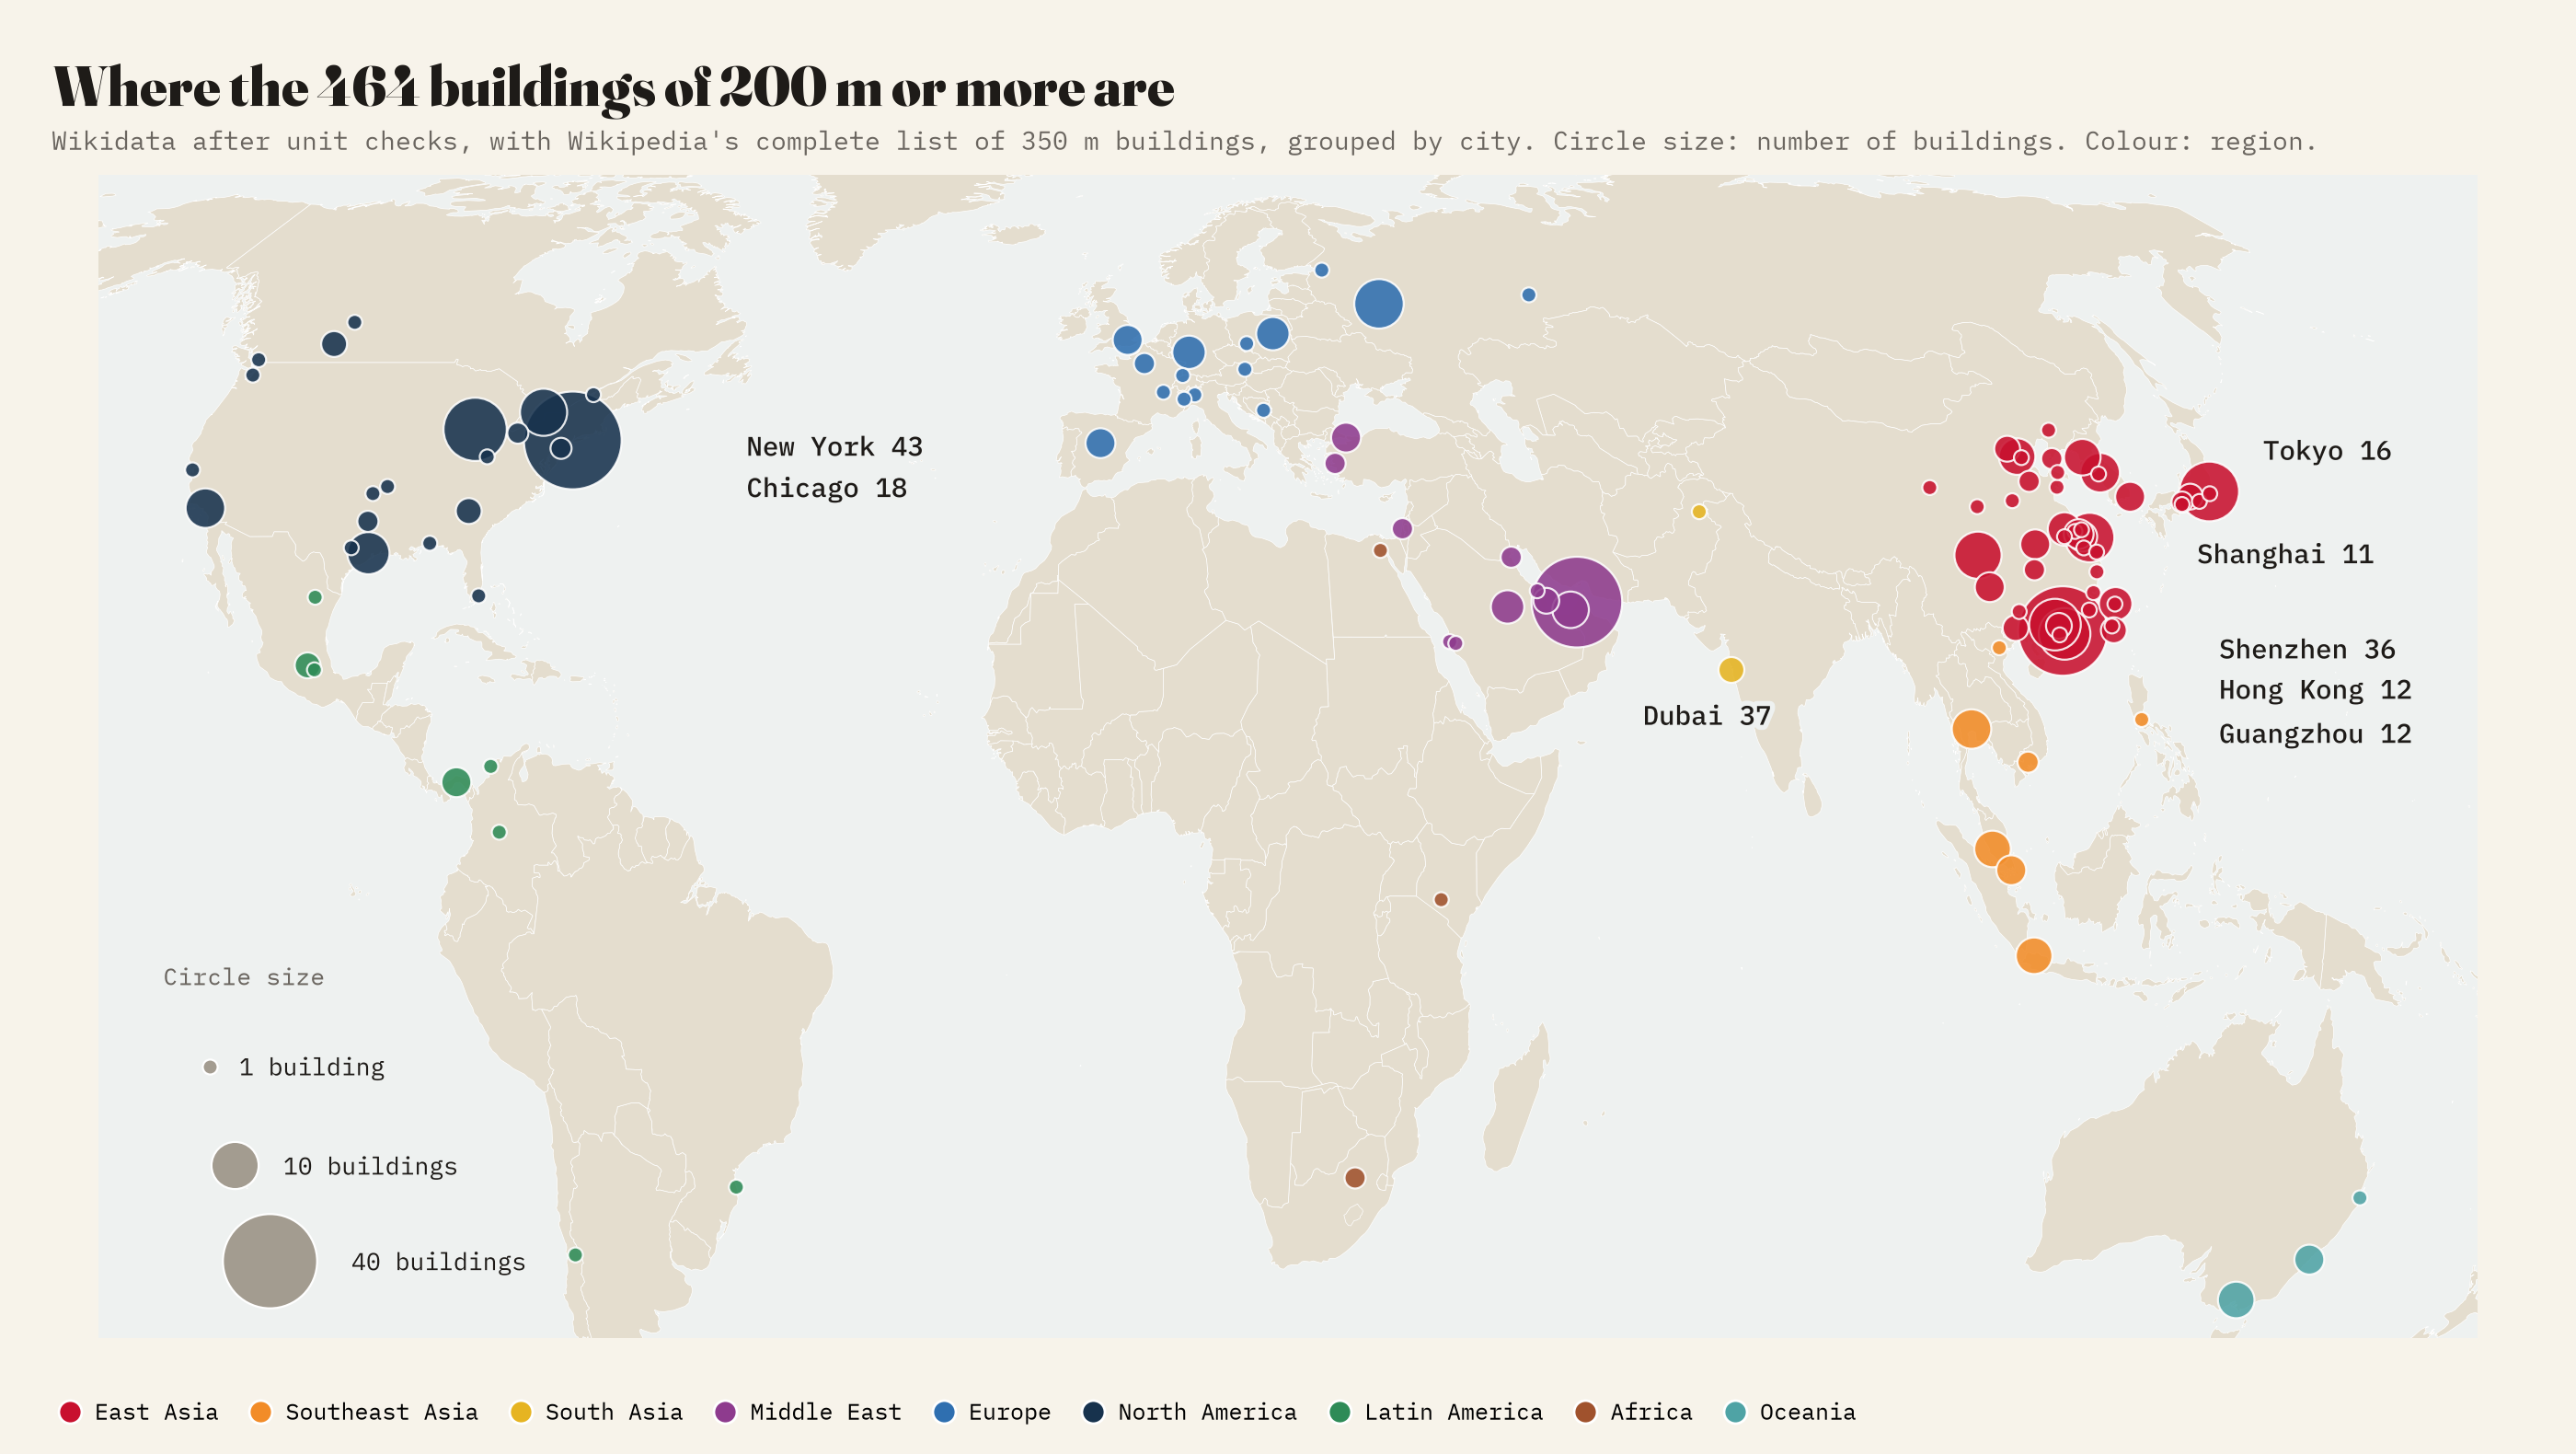
\includegraphics[width=\textwidth]{f_map200.png}
\caption{Buildings of 200 m or more, grouped by city (circle area: number of buildings; colour: region).}\label{fig:map}\end{figure}
\begin{figure}[tbp]\centering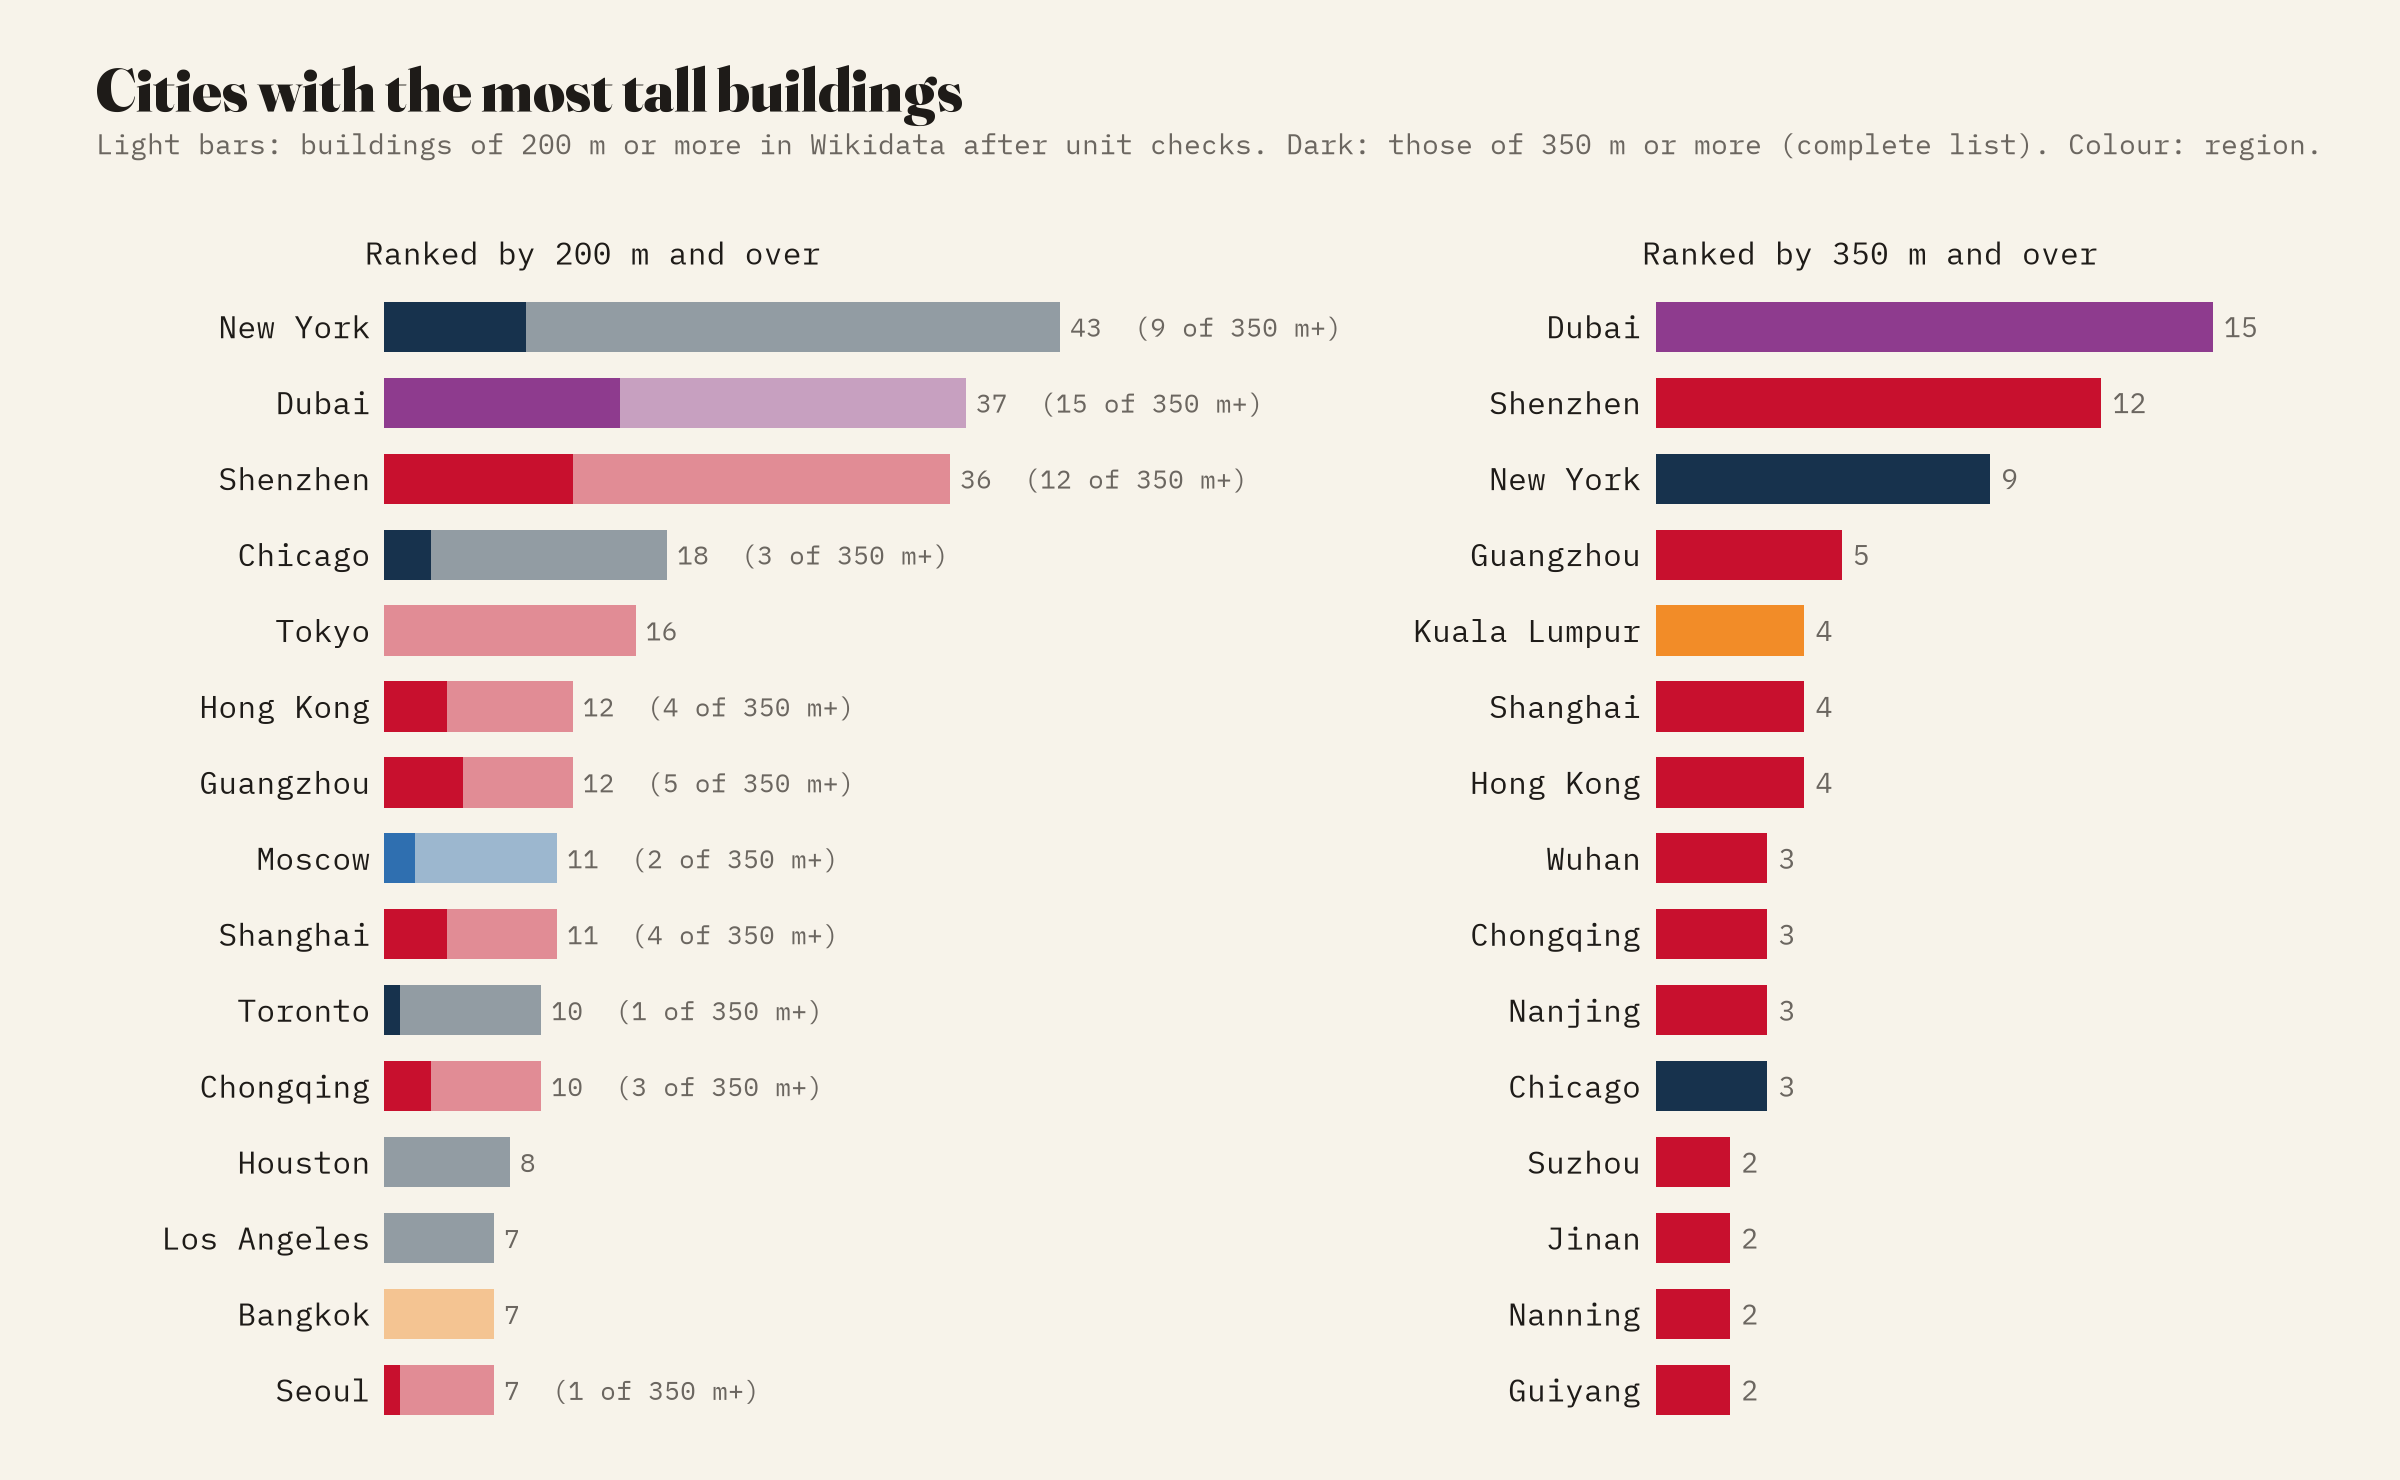
\includegraphics[width=\textwidth]{f_cities.png}
\caption{Cities with the most buildings of 200 m or more in Wikidata after checks (left; dark: those of 350 m or more) and of 350 m or more on Wikipedia's complete list (right).}\label{fig:cities}\end{figure}

\begin{table}[tbp]\centering\small\caption{The fifteen cities with the most buildings of 200 m or more in Wikidata after unit checks, with how many are 350 m or more (complete list) and the tallest.}\label{tab:top}\begin{tabular}{llrr>{\raggedright\arraybackslash}p{5.6cm}}\toprule City & Country & 200 m+ & 350 m+ & Tallest\\\midrule
New York & United States & 43 & 9 & One World Trade Center (541.3 m)\\
Dubai & United Arab Emirates & 37 & 15 & Burj Khalifa (828 m)\\
Shenzhen & China & 36 & 12 & Ping An Finance Centre (599.1 m)\\
Chicago & United States & 18 & 3 & Willis Tower (442.1 m)\\
Tokyo & Japan & 16 & 0 & Azabudai Hills Mori JP Tower (325.2 m)\\
Hong Kong & Hong Kong & 12 & 4 & International Commerce Centre (484 m)\\
Guangzhou & China & 12 & 5 & Guangzhou CTF Finance Centre (530 m)\\
Moscow & Russia & 11 & 2 & Federation Tower (East Tower) (373.7 m)\\
Shanghai & China & 11 & 4 & Shanghai Tower (632 m)\\
Toronto & Canada & 10 & 1 & SkyTower at Pinnacle One Yonge (351.4 m)\\
Chongqing & China & 10 & 3 & International Land-Sea Center (458 m)\\
Houston & United States & 8 & 0 & JPMorgan Chase Tower (305.4 m)\\
Los Angeles & United States & 7 & 0 & U.S. Bank Tower (310.3 m)\\
Bangkok & Thailand & 7 & 0 & King Power Mahanakhon (314 m)\\
Seoul & South Korea & 7 & 1 & Lotte World Tower (554.5 m)\\
\bottomrule\end{tabular}\end{table}

\subsection{What comes next}
The list page shows 46 buildings of 350 m or more under construction, 42 of them in Asia and 29 in China; 1 is in the United States. Two would pass 600 m: Jeddah Tower in Saudi Arabia, with a planned architectural height of 1,008 m, 167+ floors and completion planned for 2028, and Dubai's Burj Azizi (725 m, planned for 2030). If Jeddah Tower is completed as planned it will be 180 m taller than the Burj Khalifa. I report only the page's status and planned figures; planned heights and dates often change.

\begin{table}[tbp]\centering\small\caption{The twelve tallest buildings under construction on Wikipedia's list, with planned architectural height and planned completion as the page gives them.}\label{tab:uc}\begin{tabular}{>{\raggedright\arraybackslash}p{5.2cm}>{\raggedright\arraybackslash}p{4.6cm}rr}\toprule Building & City & Height (m) & Completion\\\midrule
Jeddah Tower & Jeddah, Saudi Arabia & 1008 & 2028\\
Burj Azizi & Dubai, UAE & 725 & 2030\\
Goldin Finance 117 & Tianjin, China & 597 & 2027\\
Burj Binghatti Jacob \& Co Residences & Dubai, UAE & 557 & 2027\\
Senna Tower & Balneário Camboriú, Brazil & 550 & 2030\\
Tiger Sky Tower & Dubai, UAE & 532 & 2029\\
Six Senses Residences Dubai Marina & Dubai, UAE & 517 & 2028\\
The Line & Neom, Saudi Arabia & 500 & 2030\\
Greenland Jinmao International Finance Center & Nanjing, China & 499.8 & 2028\\
HeXi Yuzui Tower A & Nanjing, China & 498.8 & 2028\\
Panda Tower - Tianfu Center & Chengdu, China & 488.9 & 2027\\
Rizhao Center & Rizhao, China & 485 & 2028\\
\bottomrule\end{tabular}\end{table}

\section{Limitations}
The record-holder tables are Wikipedia's, and the page itself notes disputed medieval heights: Lincoln's 159.7 m is ``disputed by some, but accepted by most sources'', and Christopher Wren put Old St Paul's spire at 140 m rather than 149 m. The page is internally inconsistent in places (New York's 86 years in its introduction against 65 in its table; Taipei 101's reign ending in 2009 in the text and 2010 in the table), and the two pages disagree about Strasbourg. Dates before the 14th century are not resolved. Wikidata's heights lack units; the checks remove the worst errors but heights outside the United States are kept as given, and some will be feet. Wikidata's coverage is uneven, thinnest for China, so counts by city and region are counts of records. Inception dates are sometimes the start of construction. Buildings since demolished are not on the map. Positions of 13 list buildings are city centres, and those of Lincoln and Beauvais cathedrals were entered by hand.

\section{Conclusion}
For most of recorded history the tallest building was a church, and the longest reigns belong to Lincoln and Strasbourg rather than to any skyscraper. The skyscraper record was American for a century and has been Asian since 1998, and the tall buildings that followed are overwhelmingly Asian too. The next record, a kilometre-tall tower in Jeddah, continues that shift. Measuring the change needs care: open data can trace it, but only after the definitions are fixed and the units checked.

\section*{Data and code availability}
The interactive map is at \url{https://maps.tristanhotham.com/tallest-buildings/}. Data and code are at \url{https://github.com/Tristan-Hotham/tallest-buildings} and archived with this paper at https://doi.org/10.5281/zenodo.23857608. Tables derived from Wikipedia are released under CC BY-SA 4.0, as is the rest of the derived data; code is under the MIT licence. Wikidata is CC0. The CORGIS data were used only as a check and are not redistributed.

\section*{AI statement}
I wrote the text, with drafting and editing assistance from Claude (Anthropic), which also helped prepare the analysis code. I reviewed and checked all text and results.

\begin{thebibliography}{9}
\bibitem[CORGIS(2016)]{corgis} CORGIS Datasets Project (2016) Skyscrapers dataset, derived from the CTBUH Skyscraper Center. \url{https://github.com/corgis-edu/corgis}
\bibitem[CTBUH(2026)]{ctbuh} Council on Tall Buildings and Urban Habitat (2026) Height criteria and the Skyscraper Center. \url{https://www.ctbuh.org/}
\bibitem[Natural Earth(2026)]{naturalearth} Natural Earth (2026) Admin 0 countries and populated places. Public domain. \url{https://www.naturalearthdata.com/}
\bibitem[Šavrič et al.(2019)]{equalearth} Šavrič, B., Patterson, T. and Jenny, B. (2019) The Equal Earth map projection. \emph{International Journal of Geographical Information Science} 33(3): 454 to 465.
\bibitem[Vrandečić and Krötzsch(2014)]{wikidata} Vrandečić, D. and Krötzsch, M. (2014) Wikidata: a free collaborative knowledgebase. \emph{Communications of the ACM} 57(10): 78 to 85. Data CC0, \url{https://www.wikidata.org/}
\bibitem[Wikipedia(2026a)]{wphist} Wikipedia contributors (2026) History of the world's tallest buildings. English Wikipedia, revision 1379678838. CC BY-SA 4.0. \url{https://en.wikipedia.org/wiki/History_of_the_world's_tallest_buildings}
\bibitem[Wikipedia(2026b)]{wplist} Wikipedia contributors (2026) List of tallest buildings. English Wikipedia, revision 1376498189. CC BY-SA 4.0. \url{https://en.wikipedia.org/wiki/List_of_tallest_buildings}
\end{thebibliography}
\end{document}
